\begin{frame}{Prototype réalisé}
    Prototype à l'aide de Docker et TravisCI:
    \begin{itemize}
        \item Déploiement d'un conteneur Docker avec ActiveMQ v5.12.0 sous Ubuntu 15.10;
        \item Intégration continue avec TravisCI basé sur un dépôt GitHub public;
        \item Téléchargement du conteneur depuis Docker Hub, lancement de celui-ci;
        \item Vérification de l’accessibilité de la console web et du broker JMS.
    \end{itemize}
\end{frame}

\begin{frame}{Build avec succès}
    \begin{figure}[H]
        \centering
        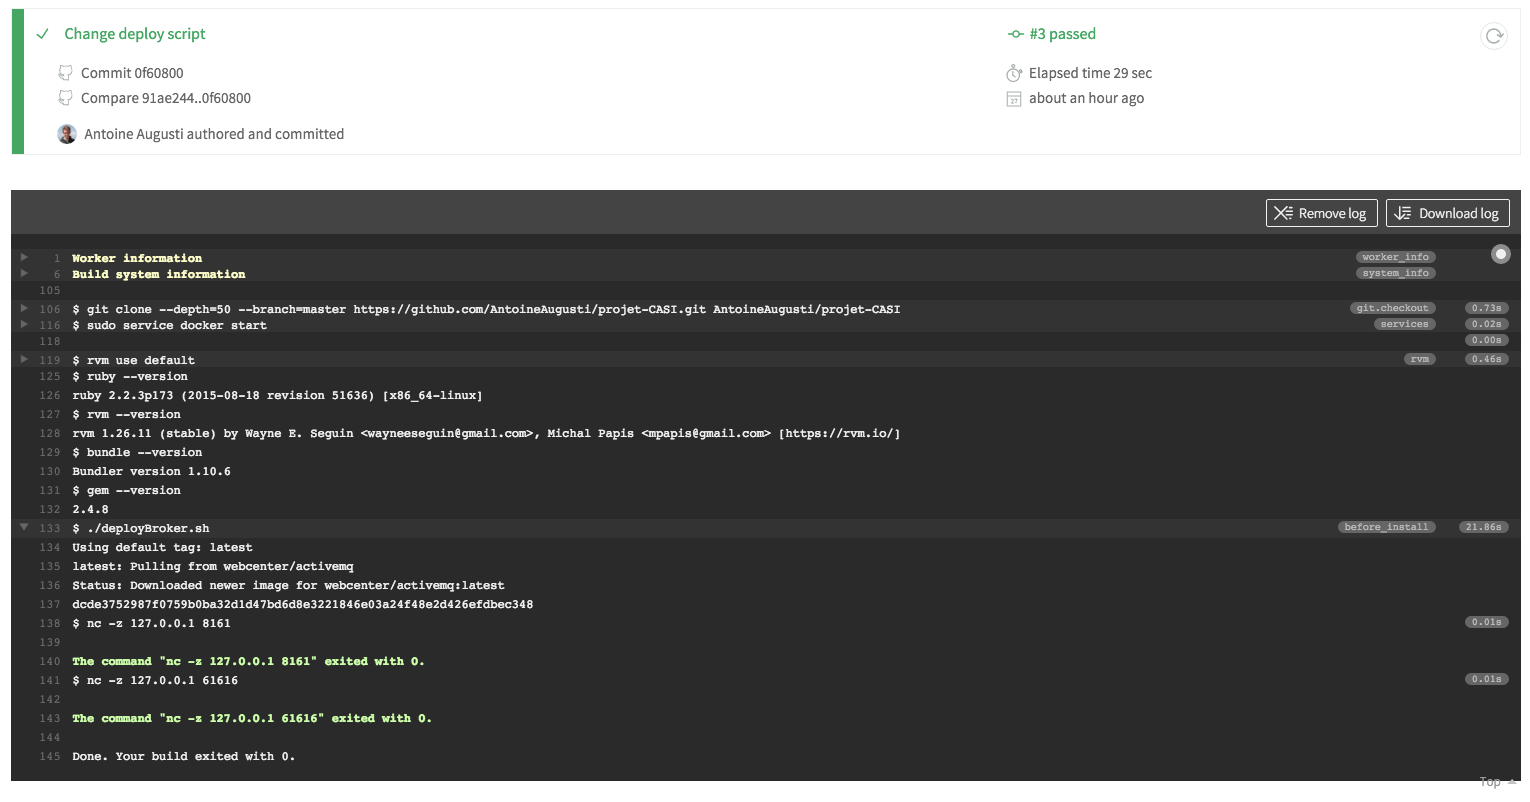
\includegraphics[width=\textwidth]{images/travis-build-success.png}
        \caption{Build s'étant terminé avec succès sur TravisCI}
    \end{figure}
\end{frame}

\begin{frame}{Pull request cassant l'infrastructure}
    \begin{figure}[H]
        \centering
        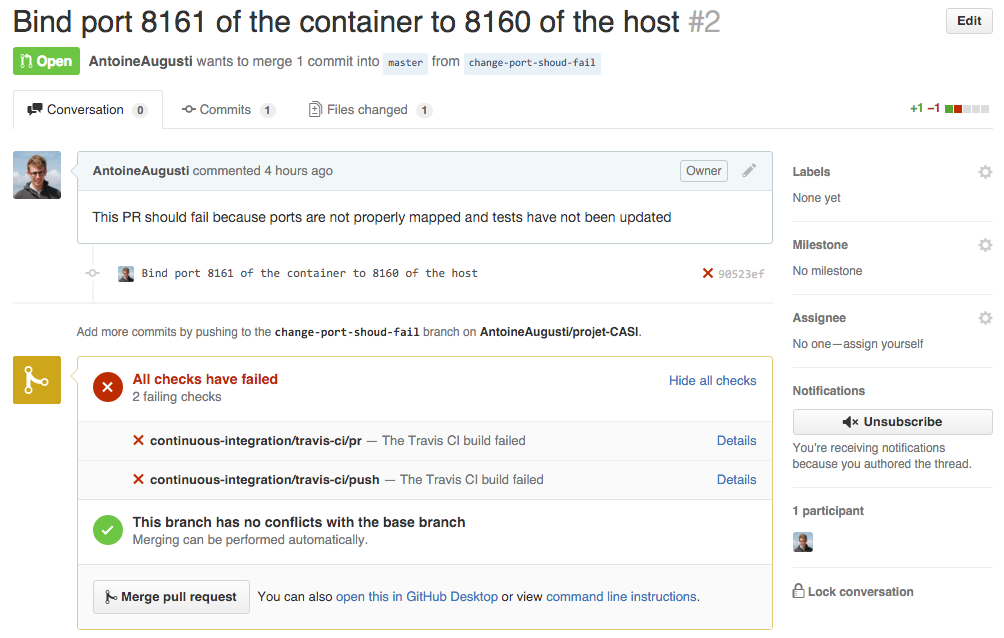
\includegraphics[width=0.8\textwidth]{images/pr-build-fail.png}
        \caption{Pull request mappant le port 8161 du conteneur sur le 8160 de la machine hôte}
    \end{figure}
\end{frame}

\begin{frame}{Build soldé par un échec}
    \begin{figure}[H]
        \centering
        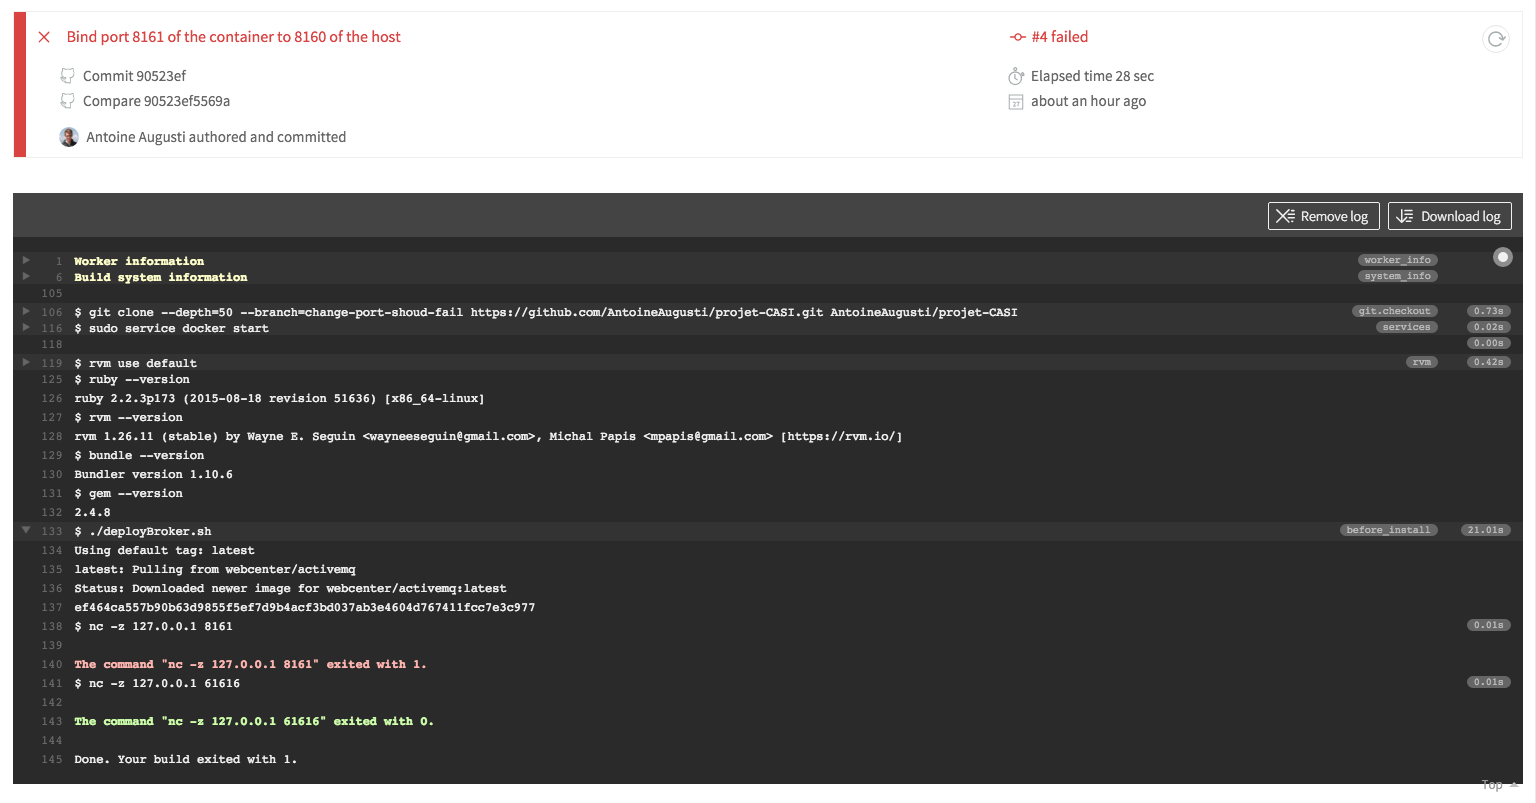
\includegraphics[width=\textwidth]{images/travis-build-failure.png}
        \caption{Build s'étant soldé par un échec sur TravisCI}
    \end{figure}
\end{frame}

\begin{frame}{Ce qu'il est possible d'assurer grâce à ce prototype}
    Ce prototype et ces tests assurent:
    \begin{itemize}
        \item Le déploiement d'un broker JMS sur plusieurs architectures: machine de développeur, intégration continue, staging, production\dots;
        \item La possibilité de déployer ce conteneur (disponibilité sur Docker Hub et fonctionnement des commandes);
        \item Le bon fonctionnement d'une configuration réseau basique.
    \end{itemize}\bigskip
    Et tout ceci est vérifié à chaque \texttt{git push} ! Il reste à intégrer avec une application productrice et une application consommatrice de messages depuis le broker JMS.
\end{frame}
